\documentclass[11pt,a4paper]{article}
\usepackage[margin=2.0cm]{geometry}
\usepackage[T1]{fontenc}
\usepackage[utf8]{inputenc}
\usepackage{lmodern}
\usepackage{microtype}
\usepackage{amsmath,amssymb}
\usepackage{booktabs,tabularx,array,makecell}
\usepackage{graphicx}
\usepackage{hyperref}
\usepackage{caption}
\usepackage{float}
\usepackage{enumitem}
\usepackage{titlesec}
\usepackage{fancyhdr}
\hypersetup{hidelinks}
\setlength{\parindent}{0pt}
\setlength{\parskip}{2.5pt}
\setlength{\tabcolsep}{3pt}
\titleformat{\section}{\large\bfseries}{\thesection.}{0.6em}{}
\titleformat{\subsection}{\normalsize\bfseries}{\thesubsection.}{0.5em}{}
\titlespacing*{\section}{0pt}{9pt plus 2pt}{4pt}
\titlespacing*{\subsection}{0pt}{7pt plus 2pt}{3pt}
\pagestyle{fancy}
\fancyhf{}
\fancyhead[L]{\small Team Lebmar (87) --- SafeInvest}
\fancyhead[R]{\small 2026 HKUST(GZ) MCM Problem A}
\fancyfoot[C]{\small\thepage}
\renewcommand{\headrulewidth}{0.4pt}

\captionsetup{font=small,labelfont=bf,labelsep=period}
\title{\vspace{-8mm}\textbf{SafeInvest: Cost-Aware Robo-Advice with Explicit Risk Limits and Human Review}}
\author{\textbf{Team Lebmar (87)}\\ Chengxuan YUAN}
\date{October 2026}

\begin{document}
\maketitle
\vspace{-6mm}

\begin{abstract}
\noindent
We build a transparent, cost-aware robo-advisory process for the SafeInvest synthetic
scenario set. For suitability, we use real purchasing-power growth, ordinary
return volatility, maximum real drawdown and a CVaR tail measure. A five-profile
by three-product training screen assigns Profile A to human review, B to
Conservative, C to Balanced, D to human review and E to Growth. For the Balanced
customer we build V2b, an annual exact-fee policy that holds, restores, makes a
bounded protective trade, or enters an absorbing human-review/hold state.

\smallskip
\noindent
Against the required one-third equal-weight baseline on the 60 final scenarios,
V2b lowers median real CAGR from 3.38\% to 2.35\% and P10 growth from 1.47\% to
0.87\%, but lowers median real MDD from 22.29\% to 20.02\%, P90 MDD from 39.36\%
to 28.69\% and breaches from 6/60 to 2/60; it trades in 21.22\% of decision
periods versus 100\% for the baseline. A transaction-fee stress (0--1\%) leaves
the main recommendation unchanged on development data; a pooled-support change
forces an initial Review, and +2 percentage points of inflation raises breaches
to 21/120.

\smallskip
\noindent
Applied unchanged to the other two assigned profiles on development data, the
same rule declines automatic funding at inception for B and E: the safeguard
extends as a funding gate, and only C receives bounded autonomous service. The
result is a risk--growth--service trade-off with an explicit human-review
safeguard, not a demonstration of fully autonomous 30-year advice.
\end{abstract}

\begin{table}[H]
\centering
\caption{Answers at a glance. Q1 in Section~\ref{sec:q1}, Q2 in
Section~\ref{sec:q2}, Q3 in Section~\ref{sec:q3}.}
\label{tab:glance}
\begin{tabular}{@{}>{\raggedright\arraybackslash}p{2.5cm}>{\raggedright\arraybackslash}p{12.6cm}@{}}
\toprule
Q1 Suitability & Products Conservative 25/30/45, Balanced 45/5/50, Growth
65/5/30 (equity/bond/bill). Onboarding on each profile's own horizon: A and D
have no risk-feasible product $\Rightarrow$ human review; B $\Rightarrow$
Conservative, C $\Rightarrow$ Balanced, E $\Rightarrow$ Growth. \\
\addlinespace
Q2 Policy & V2b: annual hold / rebalance / bounded protective trade / human
review, trading only on a strictly positive fee-net benefit. Versus the
equal-thirds baseline: lower tail risk (P90 MDD $-10.67$pp), fewer breaches
(2 vs 6), 36\% of the fees, but lower growth; trades in 21.22\% of periods.
Automated updates add risk-control value, not growth value. \\
\addlinespace
Q3 Reliability & Fee stress 0--1\% leaves the recommendation unchanged; pooled
support and +2pp inflation do not (they force review). Main safeguard: a
layered suitability screen, pre-funding gate and absorbing human review. \\
\bottomrule
\end{tabular}
\end{table}

\section{Data, assumptions and evaluation protocol}
\label{sec:data}

The supplied file contains 180 independent synthetic scenarios, each with 30
annual periods of nominal equity, bond and bill returns and inflation. Returns and
inflation are decimals; real wealth is nominal wealth divided by cumulative CPI.
The data are synthetic and based on historical U.S. series; they are not
historical observations or forecasts.

\paragraph{Assumptions.}
Conditions (A1)--(A5) are given by the problem statement; (C1)--(C3) are our own
modeling conventions, stated here and revisited in Section~\ref{sec:q3}.
\begin{enumerate}[leftmargin=1.6em,itemsep=0.5pt,label=\textbf{(A\arabic*)}]
\item Every account starts with 100 units in bills, with no later deposits or
withdrawals; portfolios are long-only and fully invested.
\item A trade charges 0.25\% of each destination amount moved, counted once and
deducted before that period's returns; the initial allocation is charged the
same way.
\item There are no taxes, other fees or terminal liquidation costs.
\item A decision for period $t$ uses only observations through $t-1$ of the
same scenario.
\item The questionnaire loss tolerance $L$ is a customer response and a review
trigger, never a guaranteed portfolio limit.
\end{enumerate}
\begin{enumerate}[leftmargin=1.6em,itemsep=0.5pt,label=\textbf{(C\arabic*)}]
\item Wealth is measured in purchasing power (nominal deflated by cumulative
CPI); growth and risk measures are real, not nominal.
\item Only annual endpoints are observed: intrayear highs and lows do not enter
the drawdown measure.
\item Scenarios are treated as independent and equally weighted; all
percentiles are empirical over the relevant scenario set.
\end{enumerate}

\paragraph{Account model.}
Formally, an account is a vector $x_t\in\mathbb{R}_{\ge0}^3$ of nominal asset
values at the start of period $t$, with cumulative CPI $c_t$ ($c_1=1$) and real
wealth $v_t=\mathbf{1}^{\top}x_t/c_t$. A decision replaces $x_t$ by post-trade
holdings $\tilde x_t$ satisfying the self-financing identity
\begin{equation}
\mathbf{1}^{\top}\tilde x_t+\phi_t=\mathbf{1}^{\top}x_t,
\qquad \phi_t=0.0025\,m_t,
\label{eq:account}
\end{equation}
where $m_t$ is the total destination amount moved, counted once. Returns then
act: $x_{t+1}=\tilde x_t\odot(1+r_t)$ and $c_{t+1}=c_t(1+\pi_t)$. The running
real peak and maximum drawdown are
\begin{equation}
P_t=\max_{s\le t}v_s,\qquad D_t=\max_{s\le t}\bigl(1-v_s/P_s\bigr),
\label{eq:mdd}
\end{equation}
and a \emph{breach} is the absorbing event $D_t>L$ for the customer's stated
loss tolerance $L$. The decision at $t$ is a function of the state
$(x_t,c_t,P_t,D_t)$ and of observations through $t-1$ only.

Original scenarios 1--120 are used for development and adjustment; scenarios
121--180 are the final evaluation set. The final 60 were exposed earlier in the
project, so the final comparison is a fixed-policy, \emph{nonblind} repetition,
not a fresh blind sample. We made no parameter, target or admission change after
the final run. This disclosure is material for interpreting every final number.

\section{Question 1: suitability, products and profiles}
\label{sec:q1}

\subsection{Measures}
Growth is the net real annualised log growth
$G_H=[\ln(V_H/\mathrm{CPI}_H)-\ln(100)]/H$, with CAGR $=\exp(G_H)-1$.
Ordinary fluctuation is the sample standard deviation of annual net real returns.
Large loss is the maximum real drawdown from the complete original peak
\eqref{eq:mdd}, using annual endpoints; it is positive and increasing in loss,
so larger values mean greater loss as required. Tail severity is the empirical
CVaR90 of the MDD distribution (and P90 MDD). The pair (ordinary volatility,
MDD) separates routine fluctuations from unusually large losses, and (C1)--(C3)
apply throughout: everything is measured in purchasing power.

\subsection{Products}
\begin{table}[H]
\centering
\caption{The three named products. Bill floors are target conventions for the
liquidity need, not live cash reserves.}
\begin{tabular}{@{}lrrr@{}}
\toprule
Product & Equity & Bond & Bill \\
\midrule
Conservative & 25\% & 30\% & 45\% \\
Balanced & 45\% & 5\% & 50\% \\
Growth & 65\% & 5\% & 30\% \\
\bottomrule
\end{tabular}
\end{table}
The target bill floor by liquidity is 30\% for High, 10\% for Medium and 0\% for
Low. A target floor is not a withdrawal guarantee or a persistent live-cash
balance.

\subsection{Onboarding rule}
Figure~\ref{fig:flow} gives the one-page decision flow. In words:
(1) take $H$, $L$ and liquidity; a missing or materially changed cash need is a
review trigger; (2) fix the three products and bill floors; (3) for each profile's
own horizon, evaluate each product on 1--120 with exact fees and annual target
restoration; retain a product only if its empirical $\mathrm{MDD}>L$ frequency is
at most 10\% and its target bill meets the liquidity floor; pool the profile
evidence into a common menu; (4) if no product is feasible, output Review; (5)
among feasible products retain training growth within $10^{-12}$ of the global
maximum, then minimise expected loss excess, then CVaR90, then the declared
candidate index; (6) assign the product. The 10\% is a declared service
reference, not a contest mandate or a calibrated probability.

\begin{figure}[p]
\centering
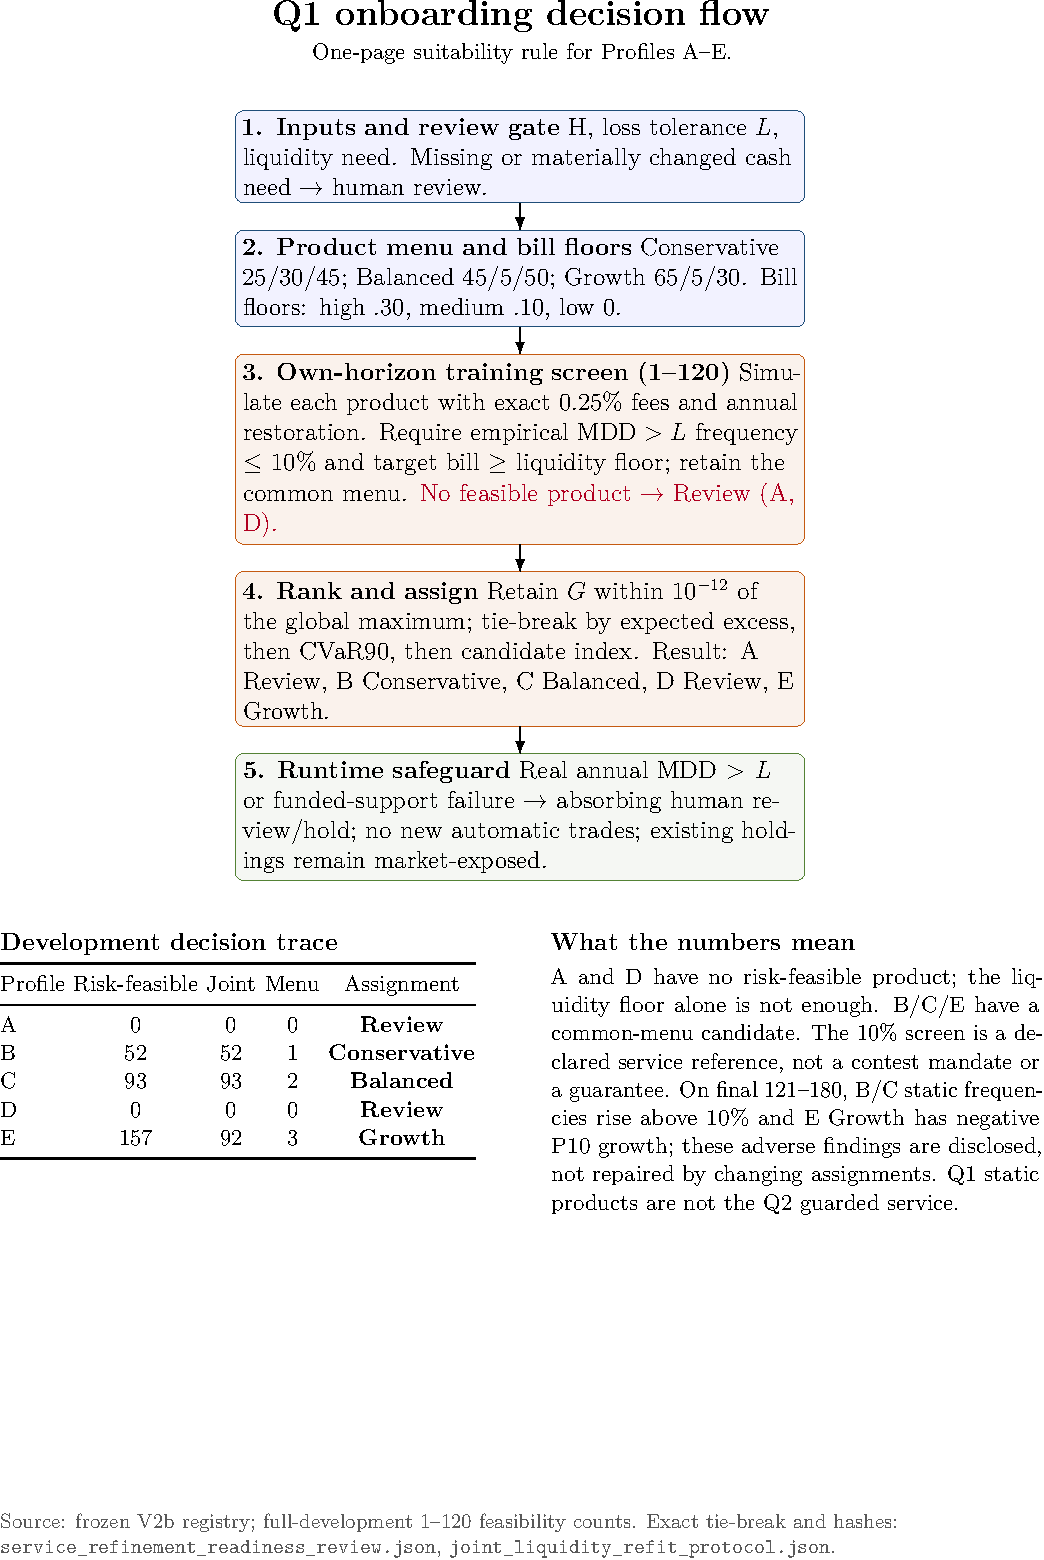
\includegraphics[width=0.93\textwidth]{figures/q1_onboarding_flow_cropped.pdf}
\caption{One-page onboarding decision flow and development decision trace. The
flow is a finite-menu rule; it is not a claim of global optimality. The 10\%
screen is an empirical training reference.}
\label{fig:flow}
\end{figure}

\subsection{The 5$\times$3 development screen}
Table~\ref{tab:fivebythree} is the 15-cell development screen. Each cell reports
median CAGR / P10 CAGR; median MDD / P90 MDD; and breaches out of 120. The bold
cell is the frozen assignment. All selected B/C/E products pass the declared 10\%
training screen (B 9/120, C 9/120, E 6/120). A and D have no risk-feasible product:
A's alternatives breach in 34--66 and D's in 67--104 of 120 paths, so the
liquidity floor alone cannot justify an allocation.

\begin{table}[H]
\centering
\caption{Development 1--120 static product screen, 5 profiles $\times$ 3 products.
Each cell: median CAGR / P10; median MDD / P90; breaches/120. Bold = frozen
assignment. This is a product screen, not the Q2 guarded service.}
\label{tab:fivebythree}
\begin{tabular}{@{}lccc@{}}
\toprule
Profile & Conservative 25/30/45 & Balanced 45/5/50 & Growth 65/5/30 \\
\midrule
A (H5, L10\%, high) & \makecell[l]{3.17 / $-$1.59\\5.56 / 14.90\\34/120} & \makecell[l]{4.36 / $-$1.85\\8.59 / 20.53\\49/120} & \makecell[l]{5.10 / $-$2.73\\11.94 / 27.46\\66/120} \\
B (H15, L25\%, medium) & \textbf{\makecell[l]{3.04 / 0.10\\13.25 / 24.22\\9/120}} & \makecell[l]{4.08 / 0.10\\17.35 / 32.65\\27/120} & \makecell[l]{5.26 / 0.02\\23.18 / 42.07\\49/120} \\
C (H30, L40\%, low) & \makecell[l]{2.97 / 1.02\\17.37 / 31.74\\1/120} & \textbf{\makecell[l]{4.03 / 1.44\\22.60 / 38.04\\9/120}} & \makecell[l]{5.12 / 1.48\\32.26 / 48.84\\35/120} \\
D (H25, L15\%, medium) & \makecell[l]{3.19 / 0.90\\16.71 / 29.37\\67/120} & \makecell[l]{4.31 / 1.34\\20.90 / 35.91\\92/120} & \makecell[l]{5.33 / 1.41\\29.18 / 47.90\\104/120} \\
E (H6, L35\%, high) & \makecell[l]{2.99 / $-$1.74\\8.08 / 18.35\\0/120} & \makecell[l]{3.75 / $-$2.33\\10.29 / 23.11\\2/120} & \textbf{\makecell[l]{5.00 / $-$3.69\\13.89 / 31.18\\6/120}} \\
\bottomrule
\end{tabular}
\end{table}

\subsection{Final assignments and own-horizon evidence}
Table~\ref{tab:profiles} evaluates the frozen assignments on final 121--180. A and
D remain Review with all financial fields NULL; they are not replaced by bills,
the baseline or a zero-risk portfolio. B/C/E use each profile's own horizon and
loss tolerance.

\begin{table}[H]
\centering
\caption{Final 121--180 own-horizon results for the frozen assignments. A/D are
unfunded Review (NULL), not zero-risk investments.}
\label{tab:profiles}
\begin{tabular}{@{}llrrrrrr@{}}
\toprule
Profile & Assignment & Target & Med. CAGR & P10 CAGR & Med. MDD & P90 MDD & Breaches \\
\midrule
A & Review & --- & NULL & NULL & NULL & NULL & NULL \\
B & Conservative & 25/30/45 & 3.21\% & 0.35\% & 14.09\% & 29.53\% & 11/60 \\
C & Balanced & 45/5/50 & 3.56\% & 1.48\% & 27.49\% & 43.54\% & 8/60 \\
D & Review & --- & NULL & NULL & NULL & NULL & NULL \\
E & Growth & 65/5/30 & 4.51\% & $-$1.58\% & 14.17\% & 31.34\% & 5/60 \\
\bottomrule
\end{tabular}
\end{table}

Briefly: A has a 5-year horizon, a 10\% loss tolerance and high liquidity; no
product passes the risk screen, so Review is the honest output. B is
Conservative: the 15-year/25\%/medium profile retains the lowest MDD and breach
frequency among its three products, and its development Conservative row passes
the 10\% screen at 9/120. C is Balanced: it buys growth over Conservative, passes
the development screen at 9/120, and the Q2 guard is the execution safeguard.
D is Review: at 25 years, 15\% loss tolerance and medium liquidity, every product
breaches 67--104 of 120 development paths. E is the most debated assignment:
Growth has the highest median CAGR (4.51\%) and a 30\% bill floor, but its final
P10 is $-$1.58\% and it breaches 5/60; the rule selects the highest-growth product
that passes the declared 10\% MDD screen, not the product with the best lower
growth tail. This is a growth-for-tail trade-off, not a guarantee.

\paragraph{Adverse tails must remain visible.}
On final data, the static B/C frequencies are 18.3\% and 13.3\%, above the 10\%
training reference; E's P10 is negative. The 10\% reference is a declared service
convention, not a contest mandate; Q1 products are static annual references, not
the Q2 guarded service. C's V2b guard reduces final breaches to 2/60. We do not
retroactively change the assignments to make the final table look better.

\subsection{Does the safeguard extend to B and E?}
\label{sec:gate}
The Q2 guard was developed for C. To test whether it is one coherent safeguard
family or a C-only device, we applied the \emph{unchanged} locked rule to B and
E with each profile's own target, horizon and $L$ on development scenarios
1--120 (a resubstitution diagnostic on data already used for development; no
final scenarios and no new fitting).

\begin{table}[H]
\centering
\caption{The unchanged execution gate at inception, development 1--120. The
budget floor is the declared convention $(1-L/2)\times v_1$ with $v_1=100$.
Only C passes; B and E enter human review before any automatic investment.}
\label{tab:gate}
\begin{tabular}{@{}llccl@{}}
\toprule
Profile & Product & $L$ & Initial floor & Gate decision \\
\midrule
B & Conservative 25/30/45 & 25\% & 87.5 & Pre-investment Review \\
C & Balanced 45/5/50 & 40\% & 80.0 & Funded (60/60 on final data) \\
E & Growth 65/5/30 & 35\% & 82.5 & Pre-investment Review \\
\bottomrule
\end{tabular}
\end{table}

Under the calendar support (Section~\ref{sec:rule}), no eligible initial
allocation exists for the Conservative or Growth targets at their floors:
every proposed allocation admits a modeled one-year outcome below the released
headroom. The safeguard is therefore one family with three consistent layers:
suitability review at onboarding (A, D), a funding gate before any automatic
investment (B, E), and bounded autonomous service only where both gates pass
(C). The static Q1 numbers of Table~\ref{tab:profiles} are suitability
references, never automatic execution approvals --- and the gate confirms this
by refusing unattended funding for B and E. Because no funded B/E guard paths
exist, this is a statement about the gate's conservatism; we claim no executed
breach reduction for these profiles. Protocol, independent audit (10{,}993
checks) and byte-exact isolated replay are in the supplementary package.

\section{Question 2: the Balanced policy}
\label{sec:q2}

\subsection{Rule}
\label{sec:rule}
For Profile C (Balanced, $H=30$, $L=40\%$, low liquidity) the strategic target is
45\% equity, 5\% bond and 50\% bills. At each annual decision the policy, which
we call V2b, can hold, restore the target, make a temporary protective exposure
proposal, make one first mitigation, or enter human review. It does not change
the strategic target: a protective proposal temporarily shifts actual holdings
toward bills, and a review/hold freezes new automatic trades. A persistent
target-update variant was evaluated and rejected
(Section~\ref{sec:value}).

\paragraph{Support and floor.}
Let $S_t=\bigl\{(1+r^{(j)}_t)/(1+\pi^{(j)}_t)\bigr\}_{j=1}^{120}$ be the
\emph{calendar support}: the real gross return vectors of the 120 development
scenarios at the same calendar year $t$. For post-trade holdings $y$, the worst
supported next-year real wealth is $\underline W_t(y)=\min_{g\in S_t} g^{\top}
y/c_t$. The client floor is $F_t=(1-L)P_t$; the budget floor releases only the
fraction $\rho=0.5$ of the remaining headroom,
\begin{equation}
B_t=\max\bigl\{F_t,\;v_t-\rho\,(v_t-F_t)\bigr\}.
\label{eq:floor}
\end{equation}

\paragraph{Candidate menu and selection.}
Thirteen actions compete at each review: hold, and for each of four tilt levels
$\tau\in\{1,0.75,0.5,0.25\}$ toward the bill corner $e_{\text{bill}}$, the exact
fee-inclusive segment from $x_t$ toward $\tau w+(1-\tau)e_{\text{bill}}$, sampled
at its two support-feasible endpoints and midpoint. An action $a$ is eligible
only if $\underline W_t(\tilde x_t(a))\ge B_t$. Among eligible actions the policy
maximizes the fee-net paired predicted log advantage over holding,
\begin{equation}
s(a)=\frac{1}{120}\sum_{j=1}^{120}\ln\frac{g_j^{\top}\tilde x_t(a)}{g_j^{\top}x_t},
\qquad g_j\in S_t,
\label{eq:score}
\end{equation}
and trades only when $s(a)>0$ strictly; ties break toward holding and lower fees.
The forecast is uniform over the same training year-$t$ real gross returns, so
the benefit test is exactly the estimated-benefit-justifies-cost condition
required by the problem; nothing is fitted on the evaluation scenarios.

\paragraph{Protection, mitigation and review.}
If holding itself violates the floor, the same menu applies but predicted growth
may be sacrificed: a protective trade is admitted only when it strictly improves
the modeled worst supported outcome after exact costs, and is labelled risk
reduction with a growth cost. If no eligible proposal exists, a one-time
nine-action mitigation menu (hold; the four tilt endpoints at fractions
$q\in\{0.5,1\}$) chooses the action maximizing $\underline W_t$ net of exact
fees, again only under strict improvement over hold, and the account then enters
absorbing human review. A realized breach $D_t>L$ at any annual endpoint also
triggers the absorbing pending-hold state. At inception the full target must
pass the same support test, otherwise the account is never funded (the gate of
Section~\ref{sec:gate}). While pending, the app holds the existing holdings,
continues market exposure and makes no new automatic trades.

\subsection{Baseline and metrics}
The required baseline is one-third equity, one-third bond and one-third bills,
restored at every review, with the same 0.25\% fee. We compare median CAGR,
median MDD, P10 CAGR, P90 MDD, breaches, trade fraction and mean nominal fees.
P10/P90 use the empirical inverse CDF; medians use the ordinary median. MDD uses
annual endpoints from the original peak and does not measure intrayear losses.

\begin{table}[H]
\centering
\caption{Final 121--180 comparison. The equal-weight baseline is the required
one-third annual-restoration rule. ``Same-target pending'' restores the Balanced
target annually until the first breach and then holds; ``same-target annual''
restores every year. Trade fraction counts periods with actual destination
movement; mean fees are nominal units per initial 100.}
\label{tab:q2}
\begin{tabular}{@{}lrrrrrrr@{}}
\toprule
Strategy & Med. CAGR & Med. MDD & P10 CAGR & P90 MDD & Breaches & Trade & Fees \\
\midrule
V2b & 2.35\% & 20.02\% & 0.87\% & 28.69\% & 2/60 & 21.22\% & 0.353 \\
Same-target pending & 3.56\% & 27.49\% & 1.50\% & 43.54\% & 8/60 & 94.56\% & 1.018 \\
Same-target annual & 3.56\% & 27.49\% & 1.48\% & 43.54\% & 8/60 & 100\% & 1.067 \\
Equal thirds & 3.38\% & 22.29\% & 1.47\% & 39.36\% & 6/60 & 100\% & 0.979 \\
\bottomrule
\end{tabular}
\end{table}

V2b has the lowest tail risk and fees, but it also has lower median growth and
lower P10 growth than the equal-weight baseline. It is not an all-metric
dominance claim. Against equal thirds, the median MDD falls by 2.27 percentage
points, P90 MDD by 10.67 points, breaches from 6 to 2, fees to about 36\% and
trading from 100\% to 21.22\%; median CAGR falls by 1.03 points and P10 by 0.59
points. The policy therefore buys drawdown and fee control with growth.

The mechanism matches the design. V2b spends most periods in hold or
pending-hold, so compounding is slower in good states; but the floor test
\eqref{eq:floor} forces de-risking exactly when the modeled one-year worst case
threatens the released headroom, and the absorbing review stops the policy from
adding new automatic exposure afterwards. The improvements therefore concentrate
in the tail columns (P90 MDD, breaches, fees) while the growth columns
deteriorate. Pending does not stop losses --- holdings remain exposed, as the
severe case below shows.

\begin{figure}[H]
\centering
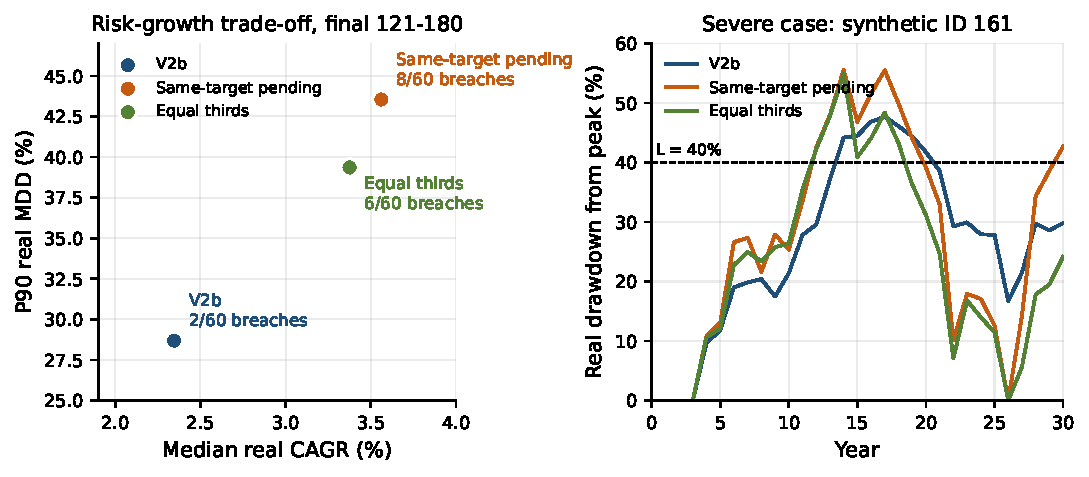
\includegraphics[width=\textwidth]{figures/q2_tradeoff_severe.pdf}
\caption{Left: final risk--growth trade-off. Right: real drawdown path of the
preselected severe synthetic case ID 161. V2b reduces the drawdown relative to
the same-target pending reference and equal thirds but still crosses the 40\%
limit.}
\label{fig:q2}
\end{figure}

\subsection{Trade frequency}
There are 382 trade periods out of 1,800 decision periods: $382/1800=21.22\%$,
including the mandatory initial allocation. Excluding the initial allocation,
$322/1740=18.51\%$. Ordinary autonomous service is a different metric:
350/1,800 $=19.44\%$ of account-years. All 60 paths enter human review by decision
year 7 (54 in year 7); the app is a bounded assisted service, not a 30-year
autonomous trader.

\subsection{Severe case and customer explanation}
The preselected severe case is synthetic ID 161, chosen by maximum main full-horizon
MDD with smallest-ID tie-break. V2b has MDD 47.68\%, CAGR $-$0.17\%, first crossing
at year 14, 20\% trade fraction and 0.236 nominal fees. Same-target pending has
55.56\%, $-$0.26\%, year 12 and 40\% trade; equal thirds has 54.84\%, $+$0.32\%,
year 12 and 100\% trade. V2b lowers drawdown versus both references but still breaches, and
its growth in this path is worse than equal thirds. The two final breaches are IDs
132 and 161, at endpoints 23 and 14; both occur after the first referral. A one-year
supported action is not a recursive or real-market safety guarantee.

The customer-facing explanation is 41 words:
\begin{quote}
Your portfolio's risk buffer no longer supports our usual trading options. We make
a protective trade only if the modeled worst outcome improves after costs, then
pause automated trading for human review. Existing holdings remain invested and
may continue losing value.
\end{quote}
It identifies the protective trade, the review request and the continued market
exposure. It does not promise recovery or an adviser response.

\subsection{Do automated weight updates add value?}
\label{sec:value}
They add \emph{risk-control} value, not growth value. The final comparison
(Table~\ref{tab:q2}) supports temporary protective/review updates: tail losses,
breaches and fees improve, while median and P10 growth deteriorate. For
persistent strategic \emph{target} updates the answer is no: a target-relearning
variant (V3) was evaluated as a pre-registered development ablation, and it
improved some service continuity but had small mixed growth/risk effects and
higher fees in all five repeats, so the simpler V2b was retained --- a
development simplicity judgment, not proof that target updates never help.
Across the same five development repeats V2b itself is stable: median CAGR
2.68--2.95\%, P90 MDD 29.0--29.4\% and 0--1 breaches out of 120. The final
policy is deliberately conservative: 19.44\% ordinary service, 2/60 breaches
and all 60 paths referred by year 7. We do not describe this as a successful
30-year autonomous robo-advisor.

\section{Question 3: reliability and safeguards}
\label{sec:q3}

\subsection{Transaction-fee stress}
We test known fees 0\%, 0.125\%, 0.25\%, 0.5\% and 1\% on the frozen V2b arm
over development 1--120. All actors know the same fee; there is no refit or new
selection. The main recommendation does not change: breaches stay 0/120 and
median CAGR moves from 2.865\% to 2.802\%; P90 MDD stays near 28.98\%. Trading
and fees move modestly. This is a cost-magnitude test, not a test of fee
misestimation, refitting or real-market safety.

\begin{table}[H]
\centering
\caption{Development 1--120 stress tests. Pooled support and +2pp inflation are
assumption changes; the final 121--180 sample is not used here.}
\label{tab:q3}
\begin{tabular}{@{}>{\raggedright\arraybackslash}p{3.1cm}>{\raggedright\arraybackslash}p{7.8cm}@{\hspace{3mm}}>{\raggedright\arraybackslash}p{3.6cm}@{}}
\toprule
Setting & V2b result & Main recommendation \\
\midrule
Fee 0--1\% & 0/120 breaches; median CAGR 2.80--2.86\%; P90 MDD $\approx$28.98\% & unchanged \\
\addlinespace
Pooled support & 0 funded; initial Review; financial NULL & changes to Review \\
Inflation +2pp & 21/120 breaches; median CAGR 0.75\%; P10 $-$1.16\%; P90 MDD 43.54\% & suspend/review \\
\bottomrule
\end{tabular}
\end{table}

\subsection{Important limitation and trigger}
The one-year support/forecast condition is empirical and finite. It is not a
conditional return distribution, a calibrated loss probability, an intrayear
stop-loss or a future guarantee. The final 121--180 sample was exposed earlier;
it is not fresh blind validation. This is the main limitation.

The primary review trigger is a funded support-family failure or no feasible
supported action. A protective trade is allowed only if the modeled worst
next-real-wealth outcome improves after exact costs; then the account enters
absorbing human review. An annual real MDD above the customer's $L$ also triggers
review. Model/input-integrity failure or a material questionnaire/cash-needs
change triggers pre-investment review. While pending, the app holds existing
holdings, makes no new automatic trades, continues actual market exposure, CPI,
original peak/MDD and financial history, and notifies the customer and adviser.
It does not assume an adviser response, a recovery reset or a liquidation.

\section{Conclusion}

The three products are Conservative 25/30/45, Balanced 45/5/50 and Growth 65/5/30.
The onboarding rule assigns A Review, B Conservative, C Balanced, D Review and E
Growth. For the Balanced customer, the V2b policy uses protective/review updates
but does not enable persistent strategic target updates. The main safeguard is
layered and consistent: a suitability screen at onboarding, the same unchanged
support gate before any automatic funding (which admits only C), and an absorbing
human review/hold after funded-support failure or MDD above $L$ --- with no new
automatic trades while pending and existing holdings remaining exposed.

The final evidence is a trade-off, not a universal winner. V2b lowers P90 MDD,
breaches and fees relative to equal weights, but also lowers median and P10
growth, and ordinary autonomous service is only 19.44\% of account-years. The
final 121--180 sample was previously exposed; no claim of fresh blind validation
or 30-year autonomy is made. Within those limits, the result is a coherent,
explainable and risk-aware assisted service.

\paragraph{Reproducibility.}
The fixed-table adapter reproduces all 14 final objects, 840 path rows and 505
saved array fields from the supplied data. The B/E funding-gate addendum has its
own frozen protocol, an independent audit recomputing every figure directly from
the saved physical accounts (10{,}993 checks) and an isolated replay matching all
deterministic artifacts byte for byte (210 array fields). The repository's full
test suite has 1{,}545 passing tests. These checks establish implementation and
reproduction integrity; they do not establish predictive validity or a fresh
blind test.

\paragraph{Use of AI tools.}
AI assistants including OpenAI Codex and DeepSeek were used for problem
interpretation, method discussion, code drafting and debugging, synthetic
testing, numerical review and English editing. Automated numerical audits and
independent-agent reviews were used as checks, not as external human peer review.
All AI-generated content, code, calculations and references were reviewed by the
participant; Chengxuan YUAN, Team Lebmar (87), remains responsible for the
submitted work and its disclosures.

\paragraph{Data attribution.}
The SafeInvest Synthetic Dataset is based on selected United States series from
the Jordà--Schularick--Taylor Macrohistory Database, Release 6. It does not
reproduce historical observations and is not a forecast. The dataset and problem
statement are distributed for noncommercial use under CC BY-NC-SA 4.0; attribution
and share-alike conditions are retained. No new blanket open-source licence is
granted to the participant's original code.

\begin{thebibliography}{9}
\setlength{\itemsep}{1pt}
\bibitem{problem}
HKUST(GZ), \emph{2026 MCM Senior Group Problem A: SafeInvest: Building a
Trustworthy Robo-Advisor}, 2026.
\bibitem{jst}
Ò.~Jordà, M.~Schularick and A.~M.~Taylor, \emph{Macrohistory Database},
Release 6.
\end{thebibliography}

\end{document}
